In order to mimic experimental settings we can confine root growth by containers, or we can implement obstacles hindering root growth. Furthermore, periodic domains can be used to mimic field conditions. In CPlantBox the domain geometry is represented in a mesh free way using signed distance functions (SDF). A SDF returns the distance of a point to its closest boundary, with negative sign if it lies within the domain, and a positive if the point is outside of the domain. CPlantBox has auxiliary functions for creating simple domains, which is shown in the following example.

\subsubsection*{Growth in a container}

We show two examples where the plants root system grows confined by two types of containers, a cylindrical container or a rectangular rhizotron. 

\lstinputlisting[language=Python, caption=Root growth in a container (topics\_virtual.py)]{examples/topics_virtual.py}

The geometry is first created by constructing a specialization of the class {SignedDistanceFunction}, 
which is passed to the root system by the method {plant.setGeometry()}: 
\begin{itemize}
 \item[9-11] Choose the parameter input file
 \item[14] Construct a cylindrical container. 
 \item[17] Construct a rhizotron.
 \item[20] Pick one of the two geometries. Note that it is important to call plant.setGeometry() before plant.initialize().
 \item[23,24] Initializes and simulates for 40 days.
 \item[27] Exports the plant structure geometry (without the soil domain geometry).
 \item[31] Its possible to save the soil domain geometry as Paraview Python script for visualization (and debugging), see Figure \ref{fig:topics_virtual}. Run this script in Paraview by Tools$\rightarrow$Python Shell, Run Script. 
\item[34] Interactive VTK plot. The geometric boundaries can currently not be visualized in the interactive rendering. This could be achieved in VTK by creating an iso-surface of the implicit geometry given by the SDF. visualised. 
\end{itemize}

\begin{figure}
\begin{subfigure}[c]{0.5\textwidth}
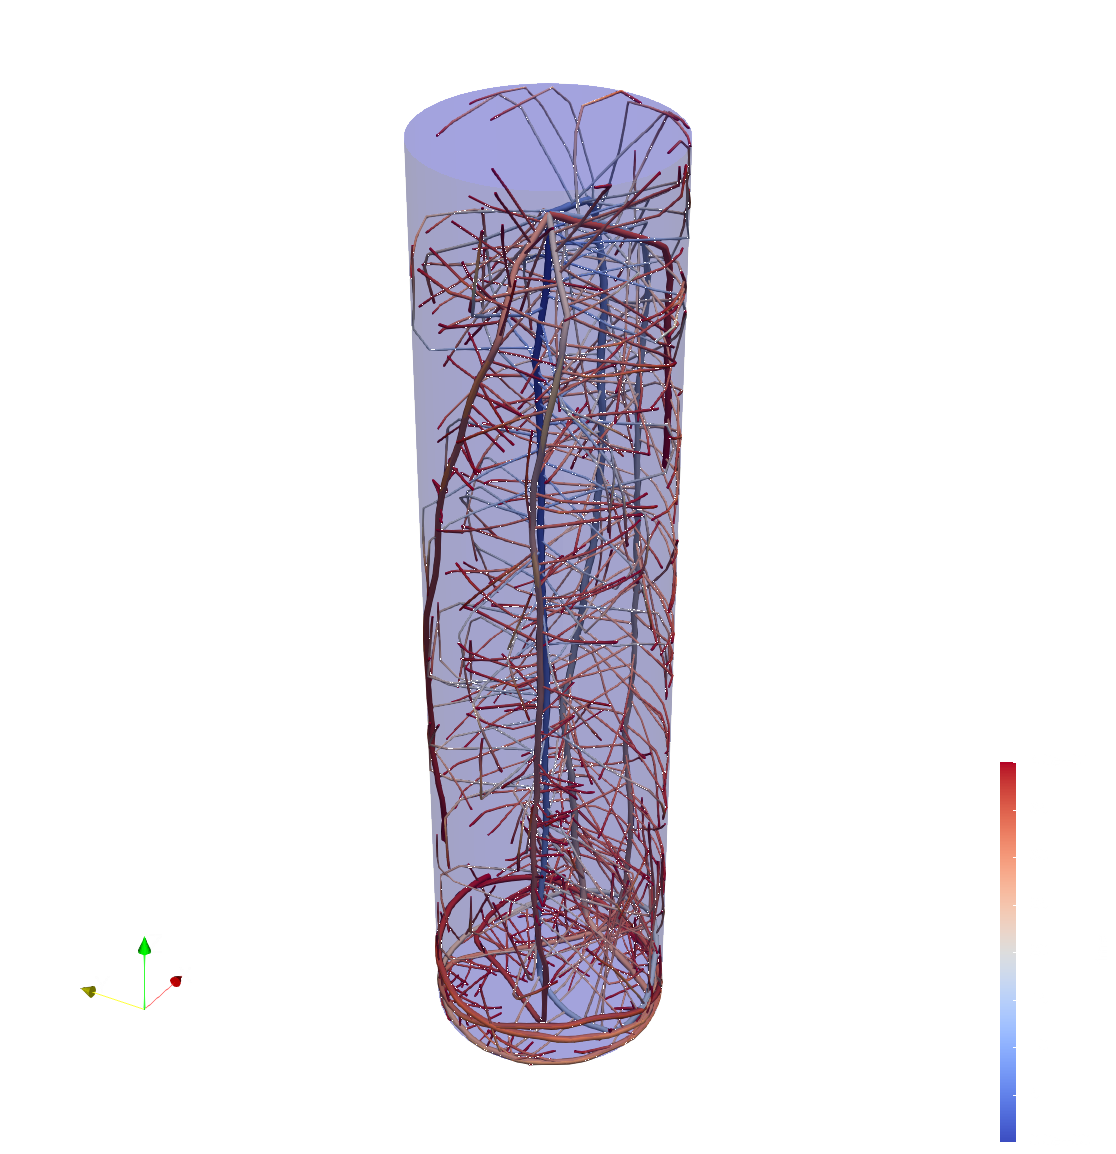
\includegraphics[width=0.99\textwidth]{figures/topics_virtual_a.png}
\subcaption{Confined by a cylinder (colour represents root age)} 
\end{subfigure}
\begin{subfigure}[c]{0.5\textwidth}
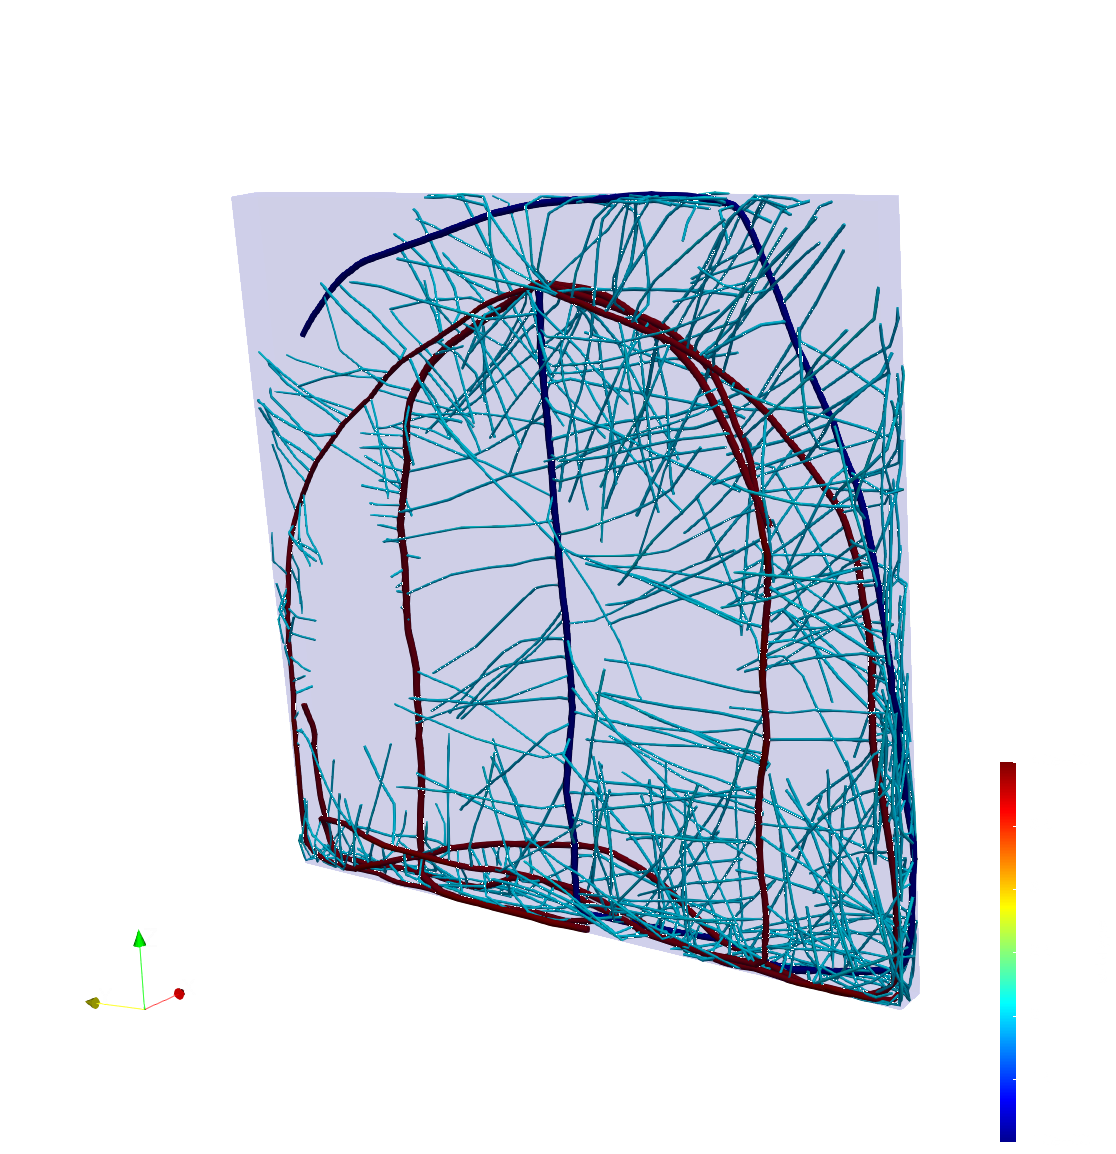
\includegraphics[width=0.99\textwidth]{figures/topics_virtual_b.png}
\subcaption{Confined by a rhizotron (colour represents root type)} 
\end{subfigure}
\caption{ParaView visualizations of results.} \label{fig:topics_virtual}
\end{figure}

Next, we show how to build more complex container geometries using SDF. 


\subsubsection*{Complex containers using SDF with set operations}

In the following example we create some geometries that we might encounter in actual experiments. First, we show how to rotate a rhizotron (e.g. to see more roots at the wall due to gravitropism). Second, we create a split box experiment, and furthermore, an example where rhizotubes act as obstacles. The following examples demonstrates how to build a complex geometry using rotations, translations and set operations on the SDF.

\lstinputlisting[language=Python, caption=Root growth in more complex containers (topics\_virtual2.py)]{examples/topics_virtual2.py}

\begin{itemize}
\item[14-19] Definition of a rotated rhizotron, see Figure \ref{fig:topics_virtual2_a}: 
L15 creates the flat container with a small height, this container is then rotated and translated into the desired position. L16 is the location of the plant seed within the unrotated rhizotron. L17 defines the rotational matrix rotating around the x-axis. In L18 the seed position is rotated. Finally, in L21 the rhizotron is rotated and translated so that the seed location is moved to the origin. 
\item[21-30] Definition of of a split box, see Figure \ref{fig:topics_virtual2_b}: 
The split box is composed of a left box, a right box, and a top box connecting left and right. 
In L30 the geometry is defined by the set operation union of the three compartments. 
\item[33] Pick one of the three geometries for your simulation.
\item[39] Also more complex geometries can be visualized by the Paraview script, 
however, set operations are not really performed, only the involved geometries are visualized.
\item[40] We cannot visualize the container geometry in the interactive rendering, but only the resulting root system. 
\end{itemize}

\begin{figure}
\begin{subfigure}[c]{0.49\textwidth}
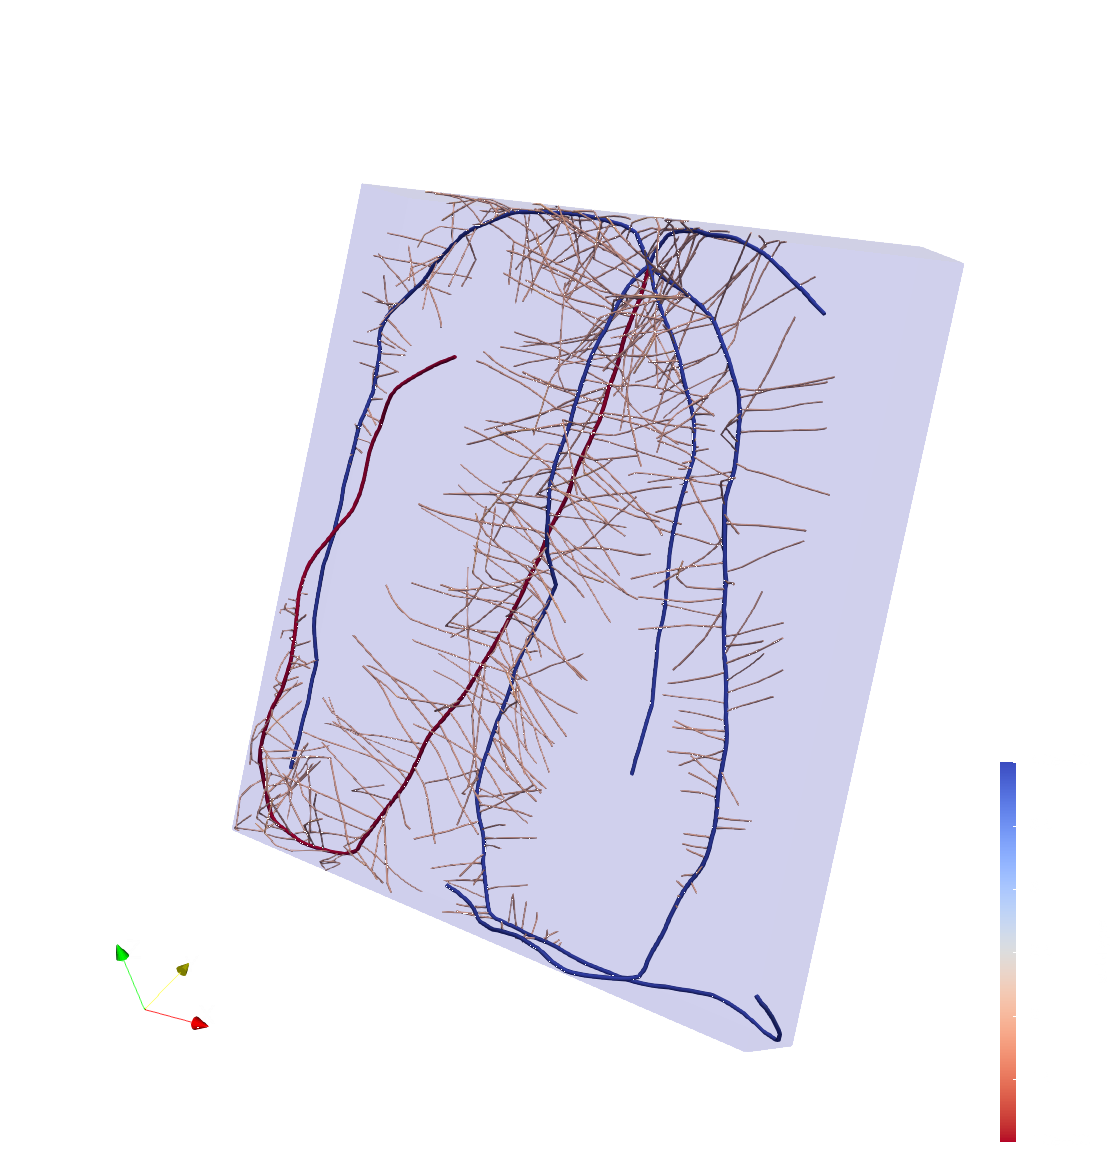
\includegraphics[width=0.99\textwidth]{figures/topics_virtual2_a.png} 
\subcaption{Rotated rhizotron} \label{fig:topics_virtual2_a}
\end{subfigure}
\begin{subfigure}[c]{0.49\textwidth}
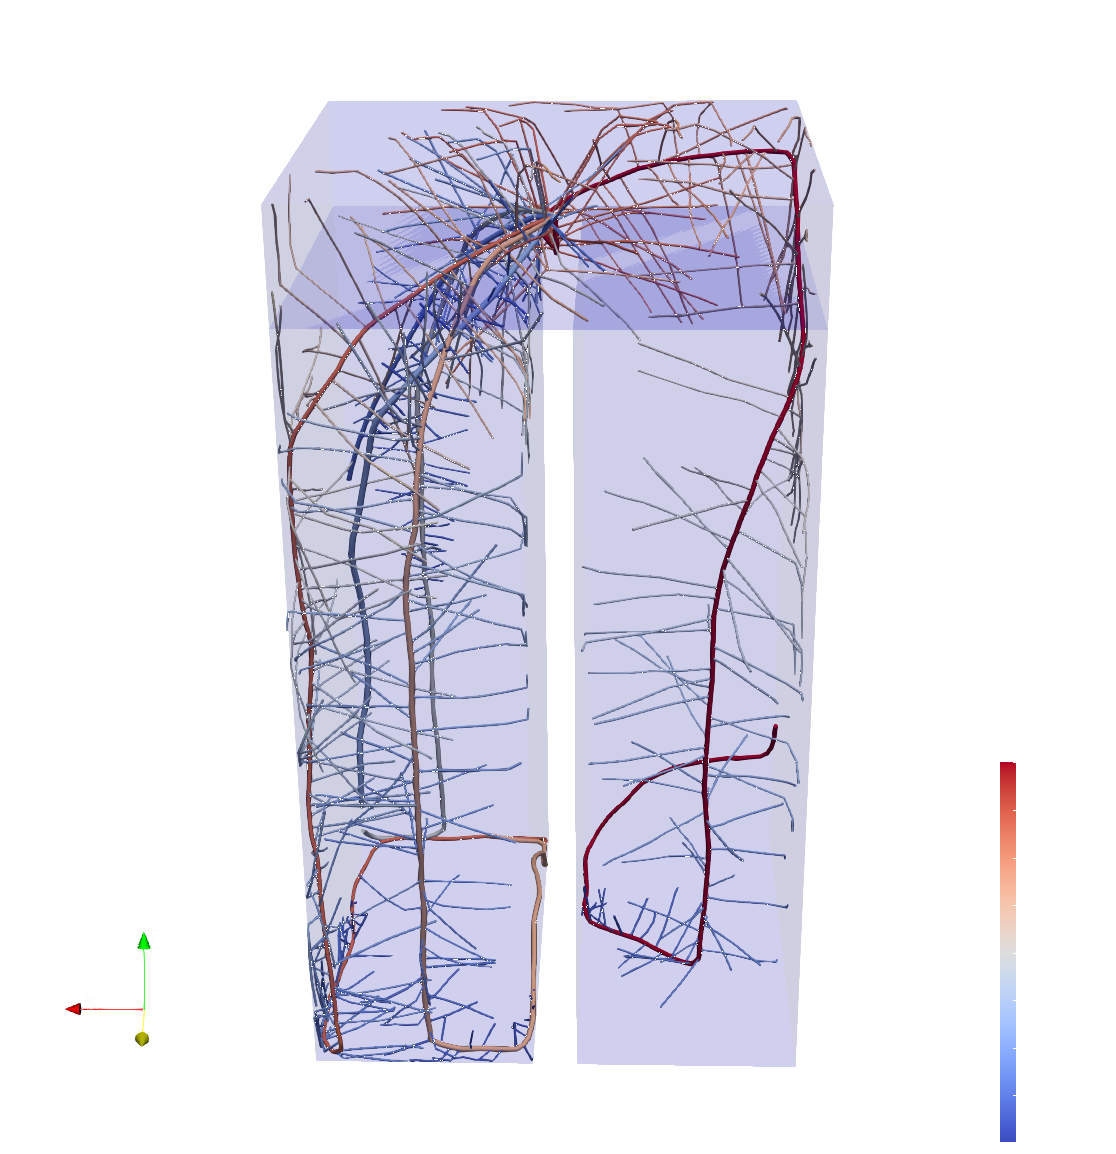
\includegraphics[width=0.99\textwidth]{figures/topics_virtual2_b.png} 
\subcaption{Split box experiment} \label{fig:topics_virtual2_b}
\end{subfigure}
\caption{Complex container geometries described by SDF and set operations.}
\end{figure}

\subsubsection*{Obstacles using SDF}

We can also use set operations to create obstacles. The following example shows a rhizotube camera setup, where transparent tubes are used to analyse root growth. We can mimic this setup by defining tubes that act as an obstacle to the growing roots. The following code is similar to before, but using another geometry: 

\lstinputlisting[language=Python, caption=Experimental setup with rhizotubes (topics\_virtual3)]{examples/topics_virtual3.py}

Definition of rhizotubes as obstacles, see Figure \ref{fig:topics_virtual3}:
\begin{itemize}
\item[14] Defines the surrounding box 
\item[15,16] Definition of a single rhizotube, that is rotated around the y-axis. 
\item[21,26] Create a list of rhizotubes at different locations that mimics the experimental setup.  
\item[27,28] Composes the final geometry by two set operation: first a union of all tubes, and then cut them out the surrounding box by taking the difference. 
\end{itemize}

\begin{figure}
\centering
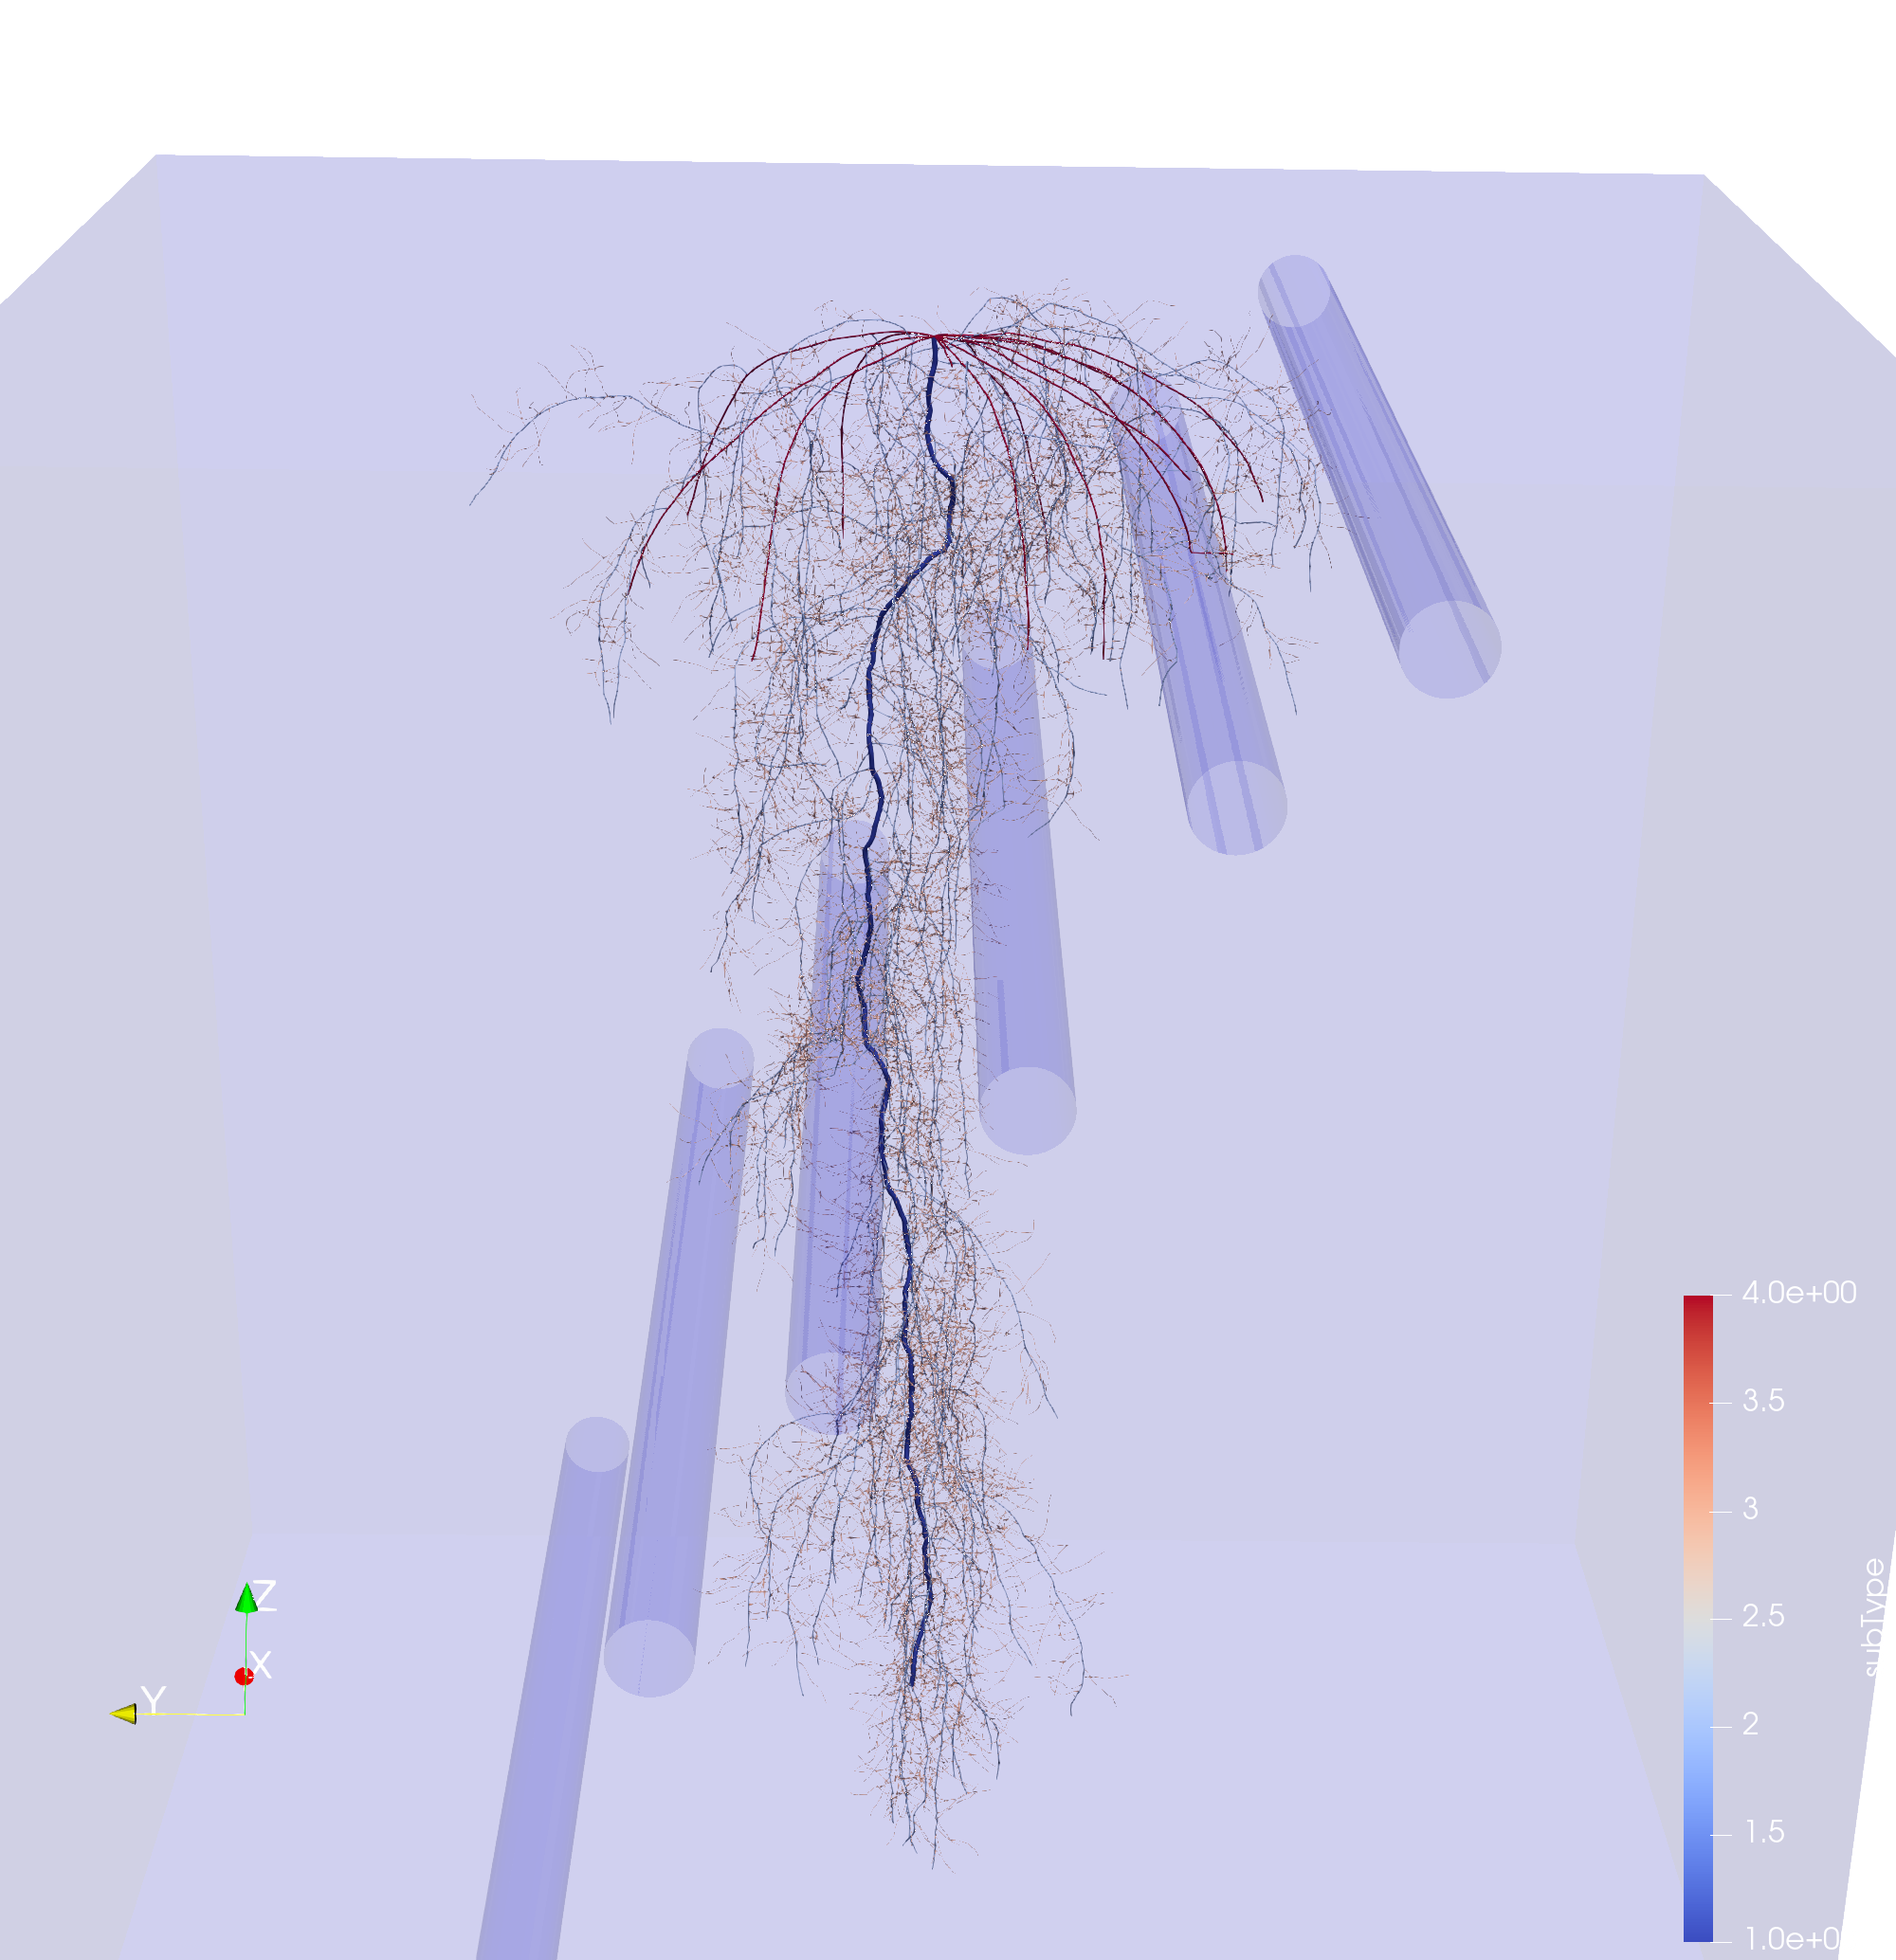
\includegraphics[width=0.7\textwidth]{figures/topics_virtual3.png}
\caption{Rhizotubes act as obstacles to the root system} \label{fig:topics_virtual3}
\end{figure}

\subsubsection*{Multiple root systems}

Its possible to simulate multiple root systems. In the following we show a small plot scale simulation:

\lstinputlisting[language=Python, caption=Multiple root systems (topics\_virtual4.py)]{examples/topics_virtual4.py}

\begin{itemize}
\item[11,12] Set the number of columns and rows of the plot, and the distance between the root systems.
\item[15-24] Creates the root systems, and puts them into a list \texttt{all}. L20 retrieves the plant seed, and L21 sets a new seed position. 
\item[26,27] Simulate all root systems.
\item[30-37] Saves each individual root systems, and additionally, saves all root systems into a single file. 
Therefore, we create an SegmentAnalyser object (see Section \ref{ssec:postprocessing}) in L30 and merge all organ segments into it (L34). Finally, we export a single VTP file (L37). The resulting geometry is shown in Figure \ref{fig:topics_virtual4}, where ParaView was used for visualisation (see Section \ref{ssec:visualisation} - ParaView).
\end{itemize}

\begin{figure}
\centering
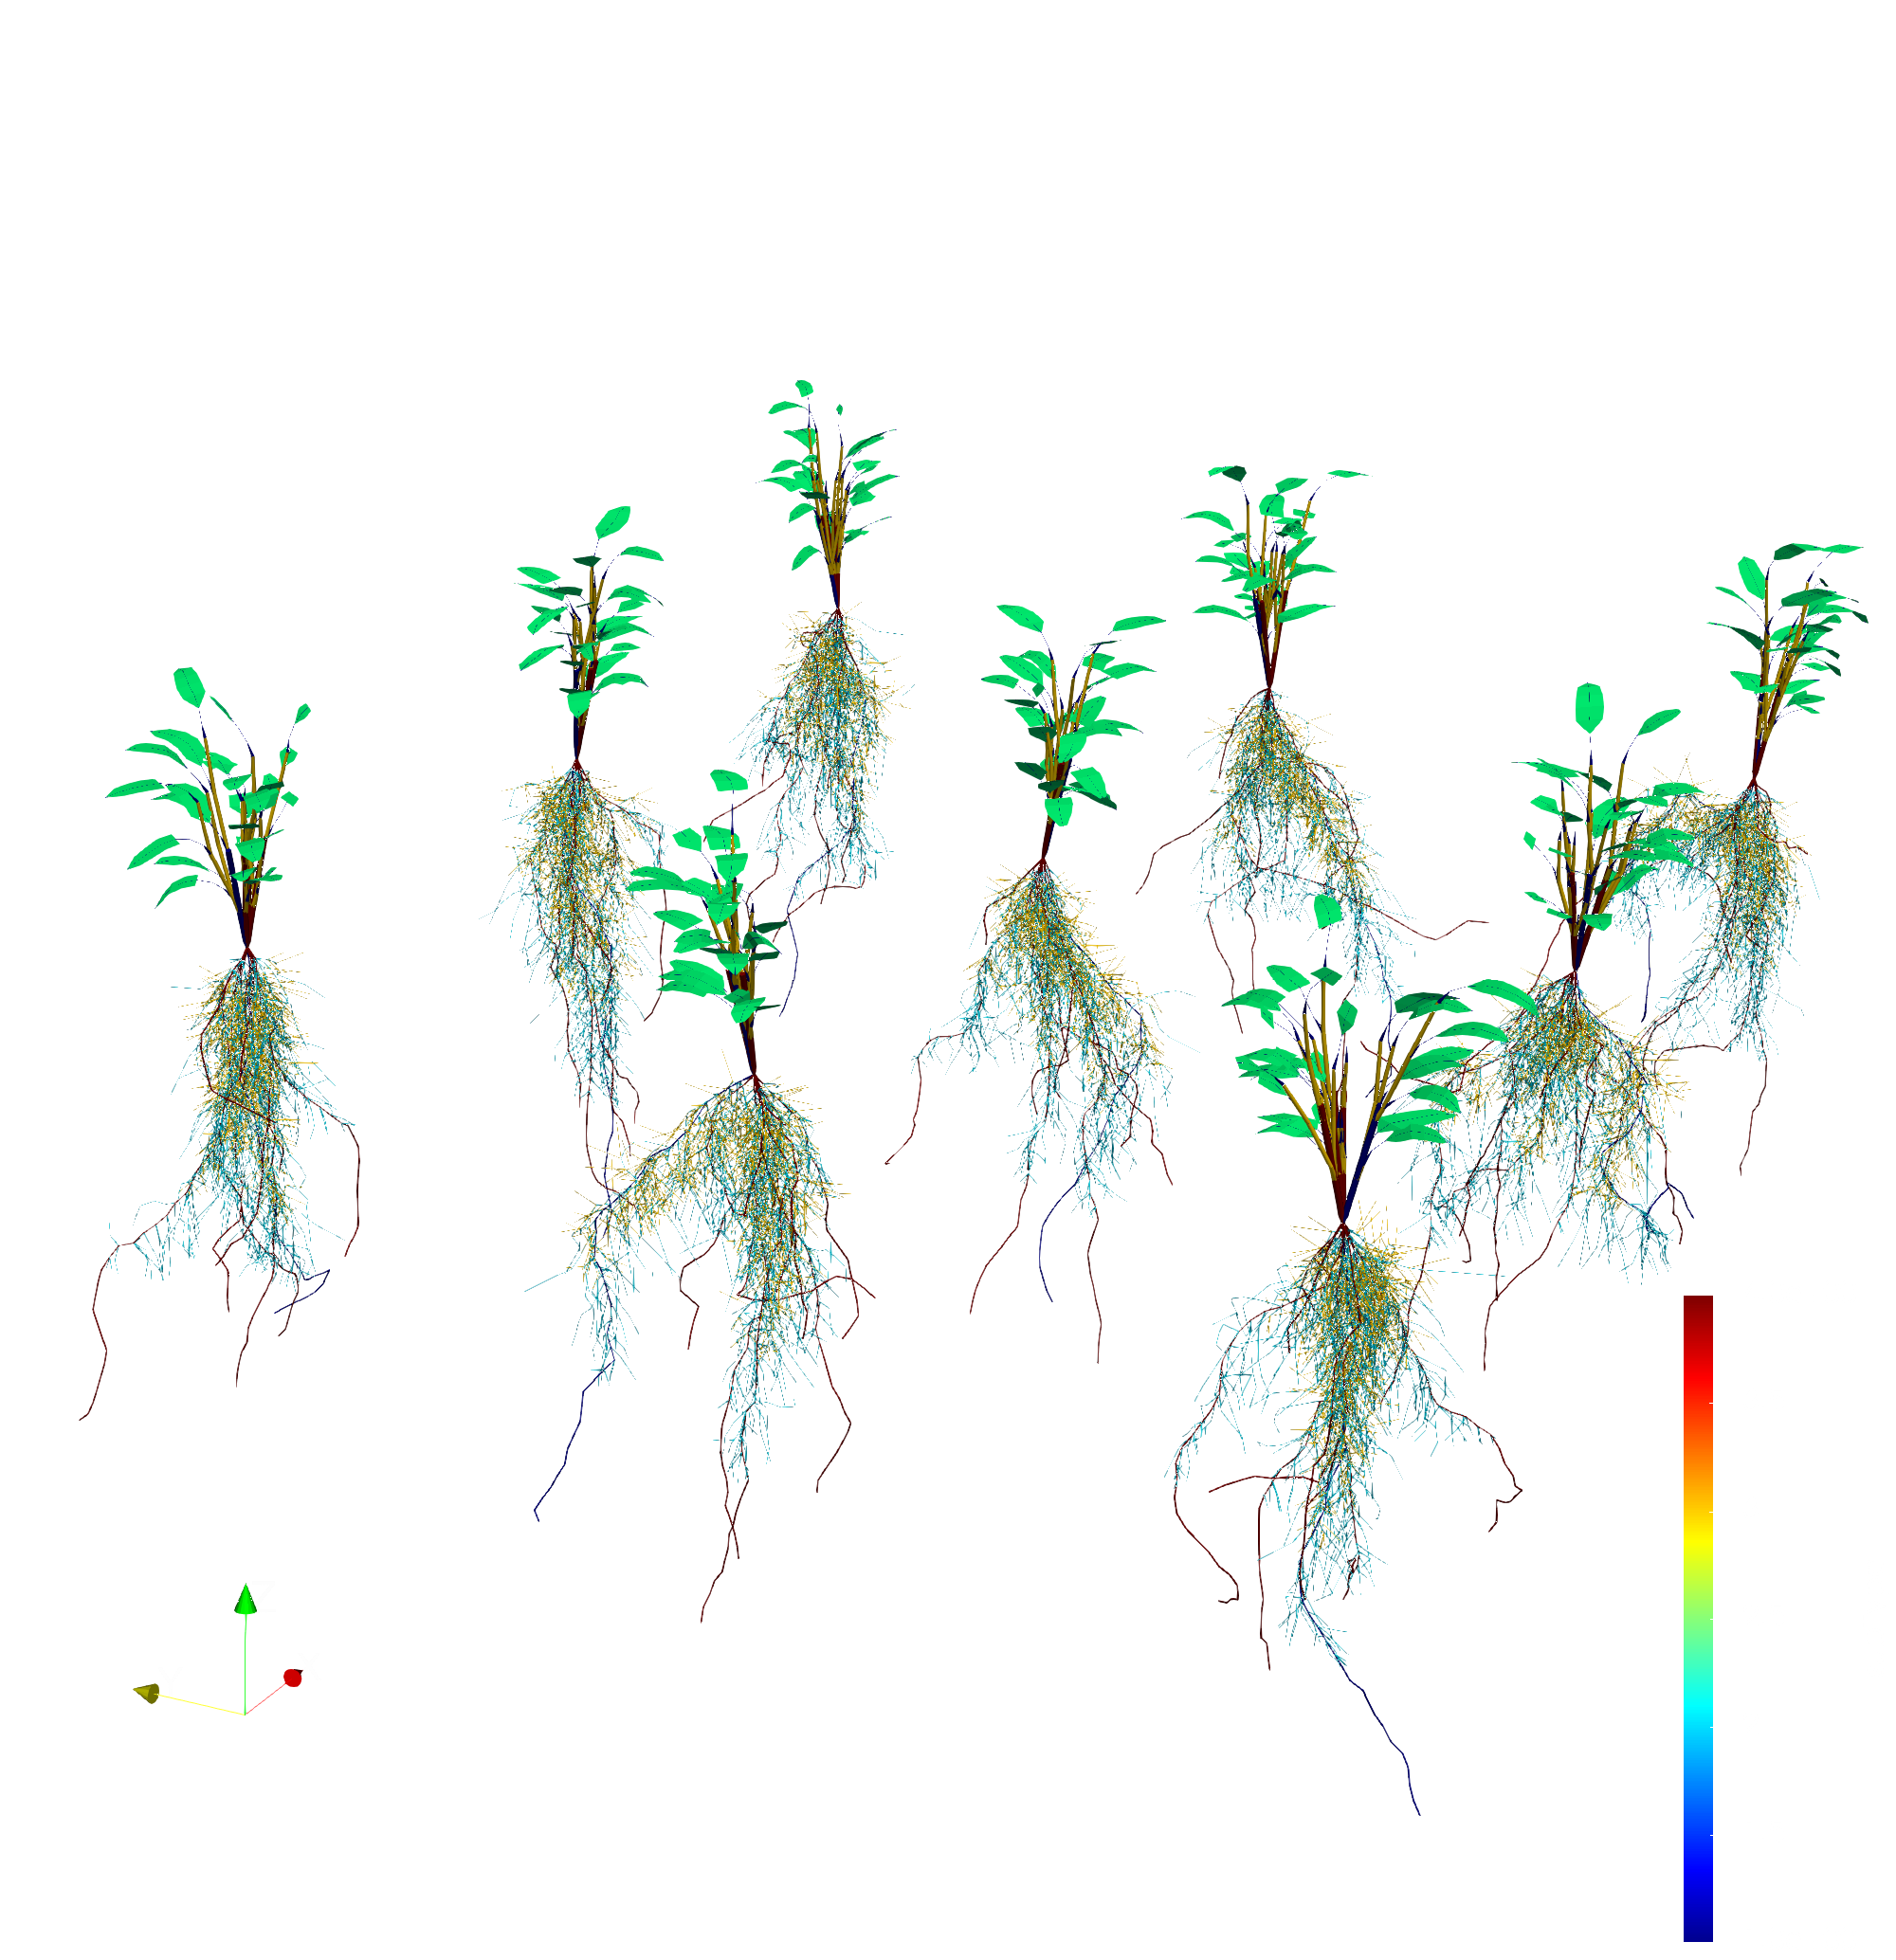
\includegraphics[width=0.7\textwidth]{figures/topics_virtual4.png}
\caption{ParaView visualization of multiple root systems.} \label{fig:topics_virtual4}
\end{figure}


\subsubsection*{Periodic domains}

If we consider only one plant type we often simplify field scale simulations to a single plant simulation with a periodic domain where the domain length and width is determined by planting density and inter-row distance. We can analyse the root geometry mapped to a periodic grid using SegmentAnalyser.mapPeriodic(), see Section \ref{ssec:postprocessing}. For coupling a root system with a periodic macroscopic soil model an unimpeded single root system is calculated and mapped into the periodic domain by the root to soil mapping function, see Section \ref{ssec:mapped}.



